\documentclass{article}

\usepackage{enumerate}
\usepackage{amssymb}
\usepackage{amsmath}
\usepackage{algorithm}
\usepackage[noend]{algpseudocode}
\usepackage{graphicx}
\usepackage{listings}

\graphicspath{ {Images/} }

\topmargin=-0.45in
\evensidemargin=0in
\oddsidemargin=0in
\textwidth=6.5in
\textheight=9.0in
\headsep=0.25in

\title{CS 189: Homework 7}
\author{Michael Stephen Chen\\ Kaggle Acct: michaelstchen \\SID: 23567341}

\begin{document}
\maketitle

\pagebreak

\section*{Problem 1: K-Means Clustering}
For K-means clustering, I randomly initialize each of the sample points to one of the $k$ clusters. The initial means are computed based on these random groupings. The updating of means/groupings terminatess when the loss no longer decreases. The loss is calculated as the sum of the squared Euclidean distances of every point from their respective cluster's mean. See \textit{digits\_kmeans.py} for the code.

\begin{enumerate}
  \item Visualization for $k=5$ clusters
    \begin{center}
      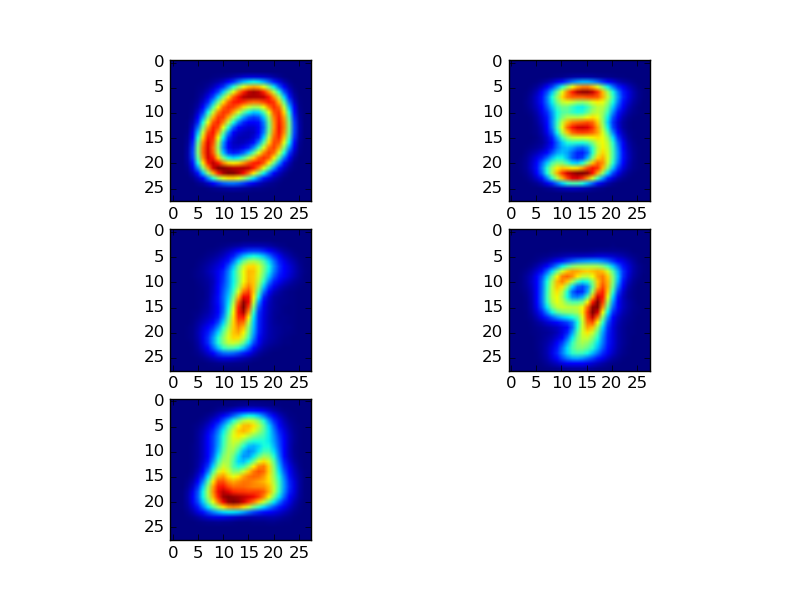
\includegraphics[scale=0.5]{kmeans_5}
    \end{center}
  \item Visualization for $k=10$ clusters
    \begin{center}
      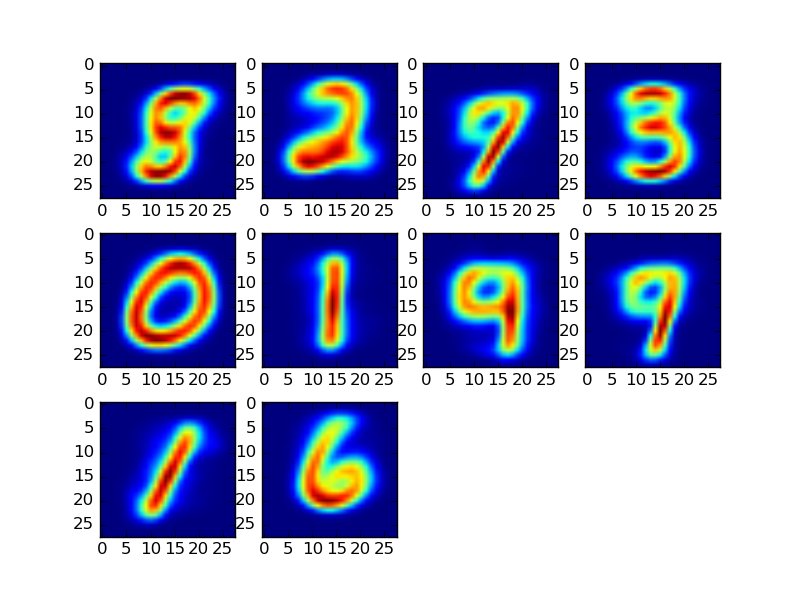
\includegraphics[scale=0.5]{kmeans_10}
    \end{center}
  \item Visualization for $k=20$ clusters
    \begin{center}
      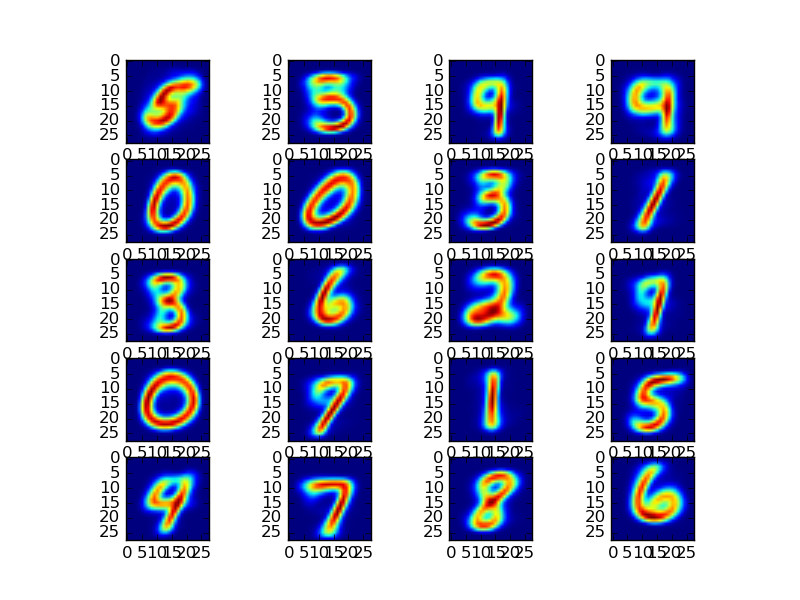
\includegraphics[scale=0.5]{kmeans_20}
    \end{center}
\end{enumerate}

The k-means does not seem to vary significantly from run to run when I randomly initialize the cluster groupings. For one run with $k=5$, I got a final k-means error of 2719265.27794. However on the subsequent run I got 2719265.19283. On the third run, I got 2719264.91943. So the exact value varies slightly from run to run, but only by a little it seems.

I noticed that some people on piazza were getting error values that are a magnitude or two larger than mine...I think it may be due to where in the iteration the error is calculated (I calculate error after updating the means but before updating the groupings). 


\section*{Problem 2: Joke Recommender System}
\begin{enumerate}
  \item \textbf{Average Rating}

    See \textit{joke\_avg.py} for the implementation. The prediction accuracy on the validation set was \textbf{0.620325}
    
  \item \textbf{K-Nearest Neighbors}

    See \textit{joke\_nn.py} for the implementation. The table below presents the results.
    \begin{center}
        $\begin{array}{c|c}
          k    & Valid Acc\\ \hline
          10   & 0.642005  \\
          100  & 0.688618 \\
          1000 & 0.694309 \\
        \end{array}$
    \end{center}
    
  For all three k-values, the validation accuracy was better than the average approach. Also the accuracy increases with increasing $k$, at least for the range of values I used.
        
  \item \textbf{Latent Factor Model}
    \begin{enumerate}
      \item See \textit{joke\_lf.py}. ``nan'' values are replaced with 0, and SVD is used to find the U (left singular vectors), D (diagonals with singular values), and V (right singular vectors) matrices.
      
      \item The MSE was calcuated for singular vector truncations to $d=2,5,10,20$. The results are presented in the table below.
        \begin{center}
        $\begin{array}{c|c|c}
          d  & MSE & Valid Acc\\ \hline
          2  & 25501804 & 0.702710\\
          5  & 25497496 & 0.679675\\
          10 & 25491425 & 0.652304\\
          20 & 25480577 & 0.598103\\
        \end{array}$
        \end{center}
        
      \item To minimize the loss function I essentially used an alternating ridge regression implemetation. For each iteration I would first solve for the $\{u_i\}$ values keeping the $\{v_j\}$ values constant, which amounted to solving the following characteristic equation:
        $$V = (U^TU + \lambda I)^{-1}U^TR$$

        Then I would solve for the $\{v_j\}$ values keeping the $\{u_i\}$ values constant, which amounted to solving the following characteristic equation:
        $$U = (V^TV + \lambda I)^{-1}V^TR^T$$

        See \textit{joke\_lfsparse.py} for the code.
        
      \item The results of the new implementation are presented below. The values were updated for 100 iterations (at which point the mse had already leveled off for quite a while). The penalty was chosenby trial and error to be $\lambda=212.5$.
        \begin{center}
        $\begin{array}{c|c|c}
          d  & MSE & Valid Acc\\ \hline
          2  & 20905131 & 0.705962\\
          5  & 19490186 & 0.720325\\
          10 & 17866870 & 0.721138\\
          20 & 15370695 & 0.710840\\
        \end{array}$
        \end{center}
        
        We see that the both the mse and the validation accuracies are higher for this new implementation as compared to the algorithm used in step 2.
    \end{enumerate}

  \item My best, and only, Kaggle submission had an accuracy of \textbf{0.70820}. The predictions were made using the sparse latent factor model with $lambda=212.5$.
\end{enumerate}

\pagebreak

\section*{Appendix: digits\_kmeans.py}
\lstinputlisting[language=python]{digits_kmeans.py}

\section*{Appendix: joke\_avg.py}
\lstinputlisting[language=python]{joke_avg.py}

\section*{Appendix: joke\_nn.py}
\lstinputlisting[language=python]{joke_nn.py}

\section*{Appendix: joke\_lf.py}
\lstinputlisting[language=python]{joke_lf.py}

\section*{Appendix: joke\_lfsparse.py}
\lstinputlisting[language=python]{joke_lfsparse.py}

\end{document}
